%%%%%%%%%%%%%%%%%%%%%%%%%%%%%%%%%%%%%%%%%
% Awesome Cover Letter
% XeLaTeX Template
% Version 1.1 (9/1/2016)
%
% This template has been downloaded from:
% http://www.LaTeXTemplates.com
%
% Original authors:
% Claud D. Park (posquit0.bj@gmail.com)
% Lars Richter (mail@ayeks.de)
% With modifications by:
% Vel (vel@latextemplates.com)
%
% License:
% CC BY-NC-SA 3.0 (http://creativecommons.org/licenses/by-nc-sa/3.0/)
%
% Important note:
% This template must be compiled with XeLaTeX, the below lines will ensure this
%!TEX TS-program = xelatex
%!TEX encoding = UTF-8 Unicode
%
%%%%%%%%%%%%%%%%%%%%%%%%%%%%%%%%%%%%%%%%%

%----------------------------------------------------------------------------------------
%	PACKAGES AND OTHER DOCUMENT CONFIGURATIONS
%----------------------------------------------------------------------------------------

\documentclass[11pt, a4paper]{awesome-cv} % A4 paper size by default, use 'letterpaper' for US letter
\usepackage[version=4]{mhchem}
\geometry{left=2cm, top=1.5cm, right=2cm, bottom=2cm, footskip=.5cm} % Configure page margins with geometry
 
\fontdir[fonts/] % Specify the location of the included fonts

% Color for highlights
\colorlet{awesome}{awesome-red} % Default colors include: awesome-emerald, awesome-skyblue, awesome-red, awesome-pink, awesome-orange, awesome-nephritis, awesome-concrete, awesome-darknight
%\definecolor{awesome}{HTML}{CA63A8} % Uncomment if you would like to specify your own color

% Colors for text - uncomment and modify
%\definecolor{darktext}{HTML}{414141}
%\definecolor{text}{HTML}{414141}
%\definecolor{graytext}{HTML}{414141}
%\definecolor{lighttext}{HTML}{414141}

\renewcommand{\acvHeaderSocialSep}{\quad\textbar\quad} % If you would like to change the social information separator from a pipe (|) to something else

%----------------------------------------------------------------------------------------
%	PERSONAL INFORMATION
%	Comment any of the lines below if they are not required
%----------------------------------------------------------------------------------------

\name{Statement of Purpose:}{UCSC}
\address{CHANG LIU\\Department of Astronomy, Peking University}

\email{ptg.cliu@pku.edu.cn}
\homepage{https://slowdiveptg.github.io}
\github{slowdivePTG}
%\skype{skypeid}
%\stackoverflow{SOid}{SOname}
%\twitter{@twit}
%\linkedin{linkedin name}
%\reddit{reddit account}
%\xing{xing name}
%\ORCID{https://orcid.org/0000-0002-7866-4531} % Other text you want to include on this line

%\position{Undergraduate Student in Astrophysics} % Your expertise/fields
%\quote{``Explore the universe, benefit the society."} % A quote or statement

\makecvfooter{\today}{Chang Liu~~~·~~~State of Purpose}{\thepage} % Specify the letter footer with 3 arguments: (<left>, <center>, <right>), leave any of these blank if they are not needed
%----------------------------------------------------------------------------------------
%	RECIPIENT/POSITION/LETTER INFORMATION
%	All of the below lines must be filled out
%----------------------------------------------------------------------------------------

\recipient{Graduate Student}{Caltech\\1200 E California Boulevard\\Pasadena, CA 91125} % The company being applied to

\letterdate{\today} % The date on the letter, default is the date of compilation

\lettertitle{Statement of Purpose} % The title of the letter

\letteropening{Dear Mr./Ms./Dr. LastName,} % How the letter is opened

\letterclosing{Sincerely,} % How the letter is closed

\letterenclosure[Attached]{Curriculum Vitae} % Any enclosures with the letter

\makecvfooter{\today}{Chang Liu~~~·~~~Statement of Purpose: UCSC}{} % Specify the letter footer with 3 arguments: (<left>, <center>, <right>), leave any of these blank if they are not needed
  
%----------------------------------------------------------------------------------------

\begin{document}

\makecvheader % Print the header

%\makelettertitle % Print the title

%----------------------------------------------------------------------------------------
%	LETTER CONTENT
%----------------------------------------------------------------------------------------

\begin{cvletter}

%------------------------------------------------

\lettersection{About Me}
As an undergraduate student in astrophysics, I have a strong urge to pursue a Ph.D degree to continue my adventure on understanding the mysteries outside our tiny planet. 

Though having been fascinated by astrophysics for long, my desire to become an astronomer, I believe, dates back in my freshman year in biology major. Though I got the \textbf{highest GPA (3.87/4)} among 120 freshmen in biology, I eventually grew tired of cumbersome taxonomy and test-tube-washing. Fortunately enough, after taking several fundamental courses on physics \& astronomy, I realized that to me, the subtle balance of astonishing physical pictures and beautiful mathematical structures is so well attained in astrophysics that I decided to switch to astronomy major. The training in School of Physics at Peking University has lain a firm foundation of \textit{mathematics} (calculus, linear algebra, PDE, and statistics) and \textit{physics} (analytical mechanics, statistical mechanics, electrodynamics, and quantum mechanics) for me. More advanced astrophysics courses (spectroscopy, cosmology, general relativity, gravitational-wave astrophysics, etc.) have equipped me for conducting research. Since my sophomore year, I have kept in \textbf{the first place in GPA (3.84/4)} among 28 students in astronomy major.

One of my greatest pursuits is to combine state-of-the-art observations with powerful computational methods to understand complex astrophysical environments. This sweet `temptation' has driven me to explore observational and computational astrophysics from various binary systems to astrochemistry within interstellar medium.

%------------------------------------------------

\lettersection{Research Experience}

My first scientific project started at the end of my second year under the supervision of \textbf{Prof. Xian Chen} in \textbf{\textit{Kavli Institute for Astronomy and Astrophysics at Peking University}} and \textbf{Prof. Fujun Du} in \textbf{\textit{Purple Mountain Observatory, Chinese Academy of Sciences}}. Starting from a `crazy' implication of recent observations that the supermassive black hole in the Milky Way was active about 2-8 Myr ago, I worked as an `archaeologist' digging out the astrochemical history of our galaxy with numerical methods. During such an ancient AGN event, tremendous hard X-ray radiation could penetrate the dusty Galactic disk, causing the synthesis of complex molecules related to the origin of life. To run the long term astrochemical simulation, I built our chemical network based on a classic gas-phase model (\href{http://faculty.virginia.edu/ericherb/research_files/osu_01_2007}{\texttt{osu\_01\_2007}}). For self-consistency, I included necessary surface processes important for molecule formation. Under a detailed AGN and galactic absorption model, I carefully embedded X-ray ionization at various distances from the galactic center in the network. The simulation was executed with the \href{http://kromepackage.org}{\texttt{KROME}} package, a widely-used library-like code for astrophysical simulation with chemistry included. We are extremely excited to see that several typical prebiotic species show observable changes in abundance distribution in the Galactic disk given former AGN events. Our paper is under final revision and will be submitted to ApJ within the next month.

My research was not limited to one single subfield. In the summer of 2019, I went to \textbf{\textit{Caltech}} as part of the Summer Undergraduate Research Fellowship (SURF) program and explored the field of transients for the first time under the mentorship of \textbf{Prof. Shrinivas Kulkarni}. With light curves from Zwicky Transient Facility (ZTF), a state-of-the-art optical time-domain survey with unprecedented field of view and survey efficiency, I conducted a systematic search for periodic white dwarf binaries. Starting with a population of 486,641 WD candidates identified in \textit{Gaia}, I performed a cross match between the so-far most complete catalog and ZTF data, selecting a subset of ~90,000 sources with over 100 observations in ZTF. My carefully designed periodogram based on the Lomb-Scargle method was then applied to the extracted light curves. A sample of 81 periodic white dwarfs (WDs) with periods between 1 and 3 hr to our surprise stood out. With combined analysis of both shapes of light curves and color information from Gaia and PanSTARRS, I classified several sources of interest including a contact binary candidate with possibly the shortest period known and an unusual strongly ellipsoidal-modulated double white dwarf system with an extremely low-mass (ELM) component. A catalog of the 81 sources with our preliminary classification has been made. Our paper will be updated with continuing follow-ups before submission to ApJ.

After an attempt to reveal the nature of various stellar systems with degenerate components in observational way, I grow intensely interested in exploring more on the intrinsic physics of compact binaries. At present I am a visiting undergraduate student at \textbf{\textit{UC Santa Cruz}} working on my thesis on the mass transfer in compact binaries with \textbf{Prof. Enrico Ramirez-Ruiz}. We focus on the so-called direct impact accretors, of which the components are white dwarfs so close to each other that the mass transfer flow from the donor strikes the accretor as opposed to forming a disk. Understanding the nature of these direct impact systems, dominant sources of GWs for space-based interferometers, will be of prime importance to next-generation detectors like \textit{LISA}. To build an intuition of mass transfer, I independently built a 3-body integrator with FORTRAN to calculate the ballistic trajectory of a particle in Roche lobe overflow in a binary system, and successfully reproduced the trajectories and angular momenta transition processes in former literature. Since then I have been conducting hydrodynamical simulations with the radiation MHD simulation code \href{http://flash.uchicago.edu/site/}{\texttt{FLASH}} to test the long-term stability of direct impact mass transfer. With the Python package \href{https://yt-project.org}{\texttt{yt}}, I have been able to visualize the torque density during mass transfer to analyze how the orbital angular momentum evolves. In the long run, we will try to work out how light curves and even gravitational radiation properties for AM CVn systems are constrained by model parameters with simulated data.

Conducting research in the most advanced facilities around the world enables me to sample various cutting-edge astronomical subfields, from astrochemistry to compact objects, and develop general skills of data analysis, visualization, and simulation on supercomputers. My proficiency in English communication and academic writing has risen to a new level after working overseas for months. More importantly, I gradually get to learn how to stay out of frustration, anxiety and loneliness, so that I am able to persist in a long-term project.
%------------------------------------------------

\lettersection{Why UCSC? - Academic Interests and Plans}
%------------------------------------------------
With unparalleled observational resources, UCSC is one of the world’s centers for astronomy. Working at UCSC as a visitor for months, I am also deeply impressed by the power of computational methods in understanding extreme astrophysical environments. UCSC highly emphasized academic training and independent research for graduate students. I would have access to diversified cutting-edge astrophysics knowledge in taking the courses as well as attending lunch talks, FLASH talks, colloquiums, and conferences. As a member of a spontaneously organized journal club of astrophysics within us undergraduate students, I deeply understand how the journal clubs on recent arXiv papers at UCSC can hone my academic presentation skills.

The 2020s' will witness the rise of time-domain and multi-messenger astronomy, especially after the first light of LSST and the launch of LISA. My experiences in observing the time-domain sky and modeling the evolution of compact binaries help to build my intense interest in the most energetic, ``breath-taking'’ events. I plan to perform my future research on various high-energy transients such as compact binaries and supernovae. I am not too surprised to find that UCSC meets so perfectly with my research experience. It would be great if I can continue working with Prof. Enrico Ramirez-Ruiz, whose excellent research covers a great breadth of computational astrophysics, including compact binary evolution, GRB triggers, and tidal events around black holes. Under his supervision, revealing the nature of compact objects with sophisticated observational properties through simulations is bound to be an exciting journey. Prof. Ryan Foley is one of the greatest supernovae hunters. I am particularly interested in electromagnetic counterparts to gravitational wave sources, of which he has rich observational experience. Besides, I also appreciate Prof. Brant Robertson’s leading work in the Computational Astrophysics Research Group, aiming at understanding the large scale structure, reionization, and intergalactic medium through advanced numerical methodologies.

I do appreciate it if you could consider my application. I am looking forward to meeting with you for a more detailed talk soon.

\begin{figure}[h]
	\centering
	\includegraphics[width=0.9\linewidth]{./h2co.pdf} 
	\caption{
		Evolution of \ce{H2CO} inside a typical molecular cloud at different Galactic distances ($1$, $2$, $4$, and $8$ kpc) after irradiated by X-ray for $10^6$ yr. 
	}
	\label{fig:1} 
\end{figure}
\begin{figure}[h]
	\centering
	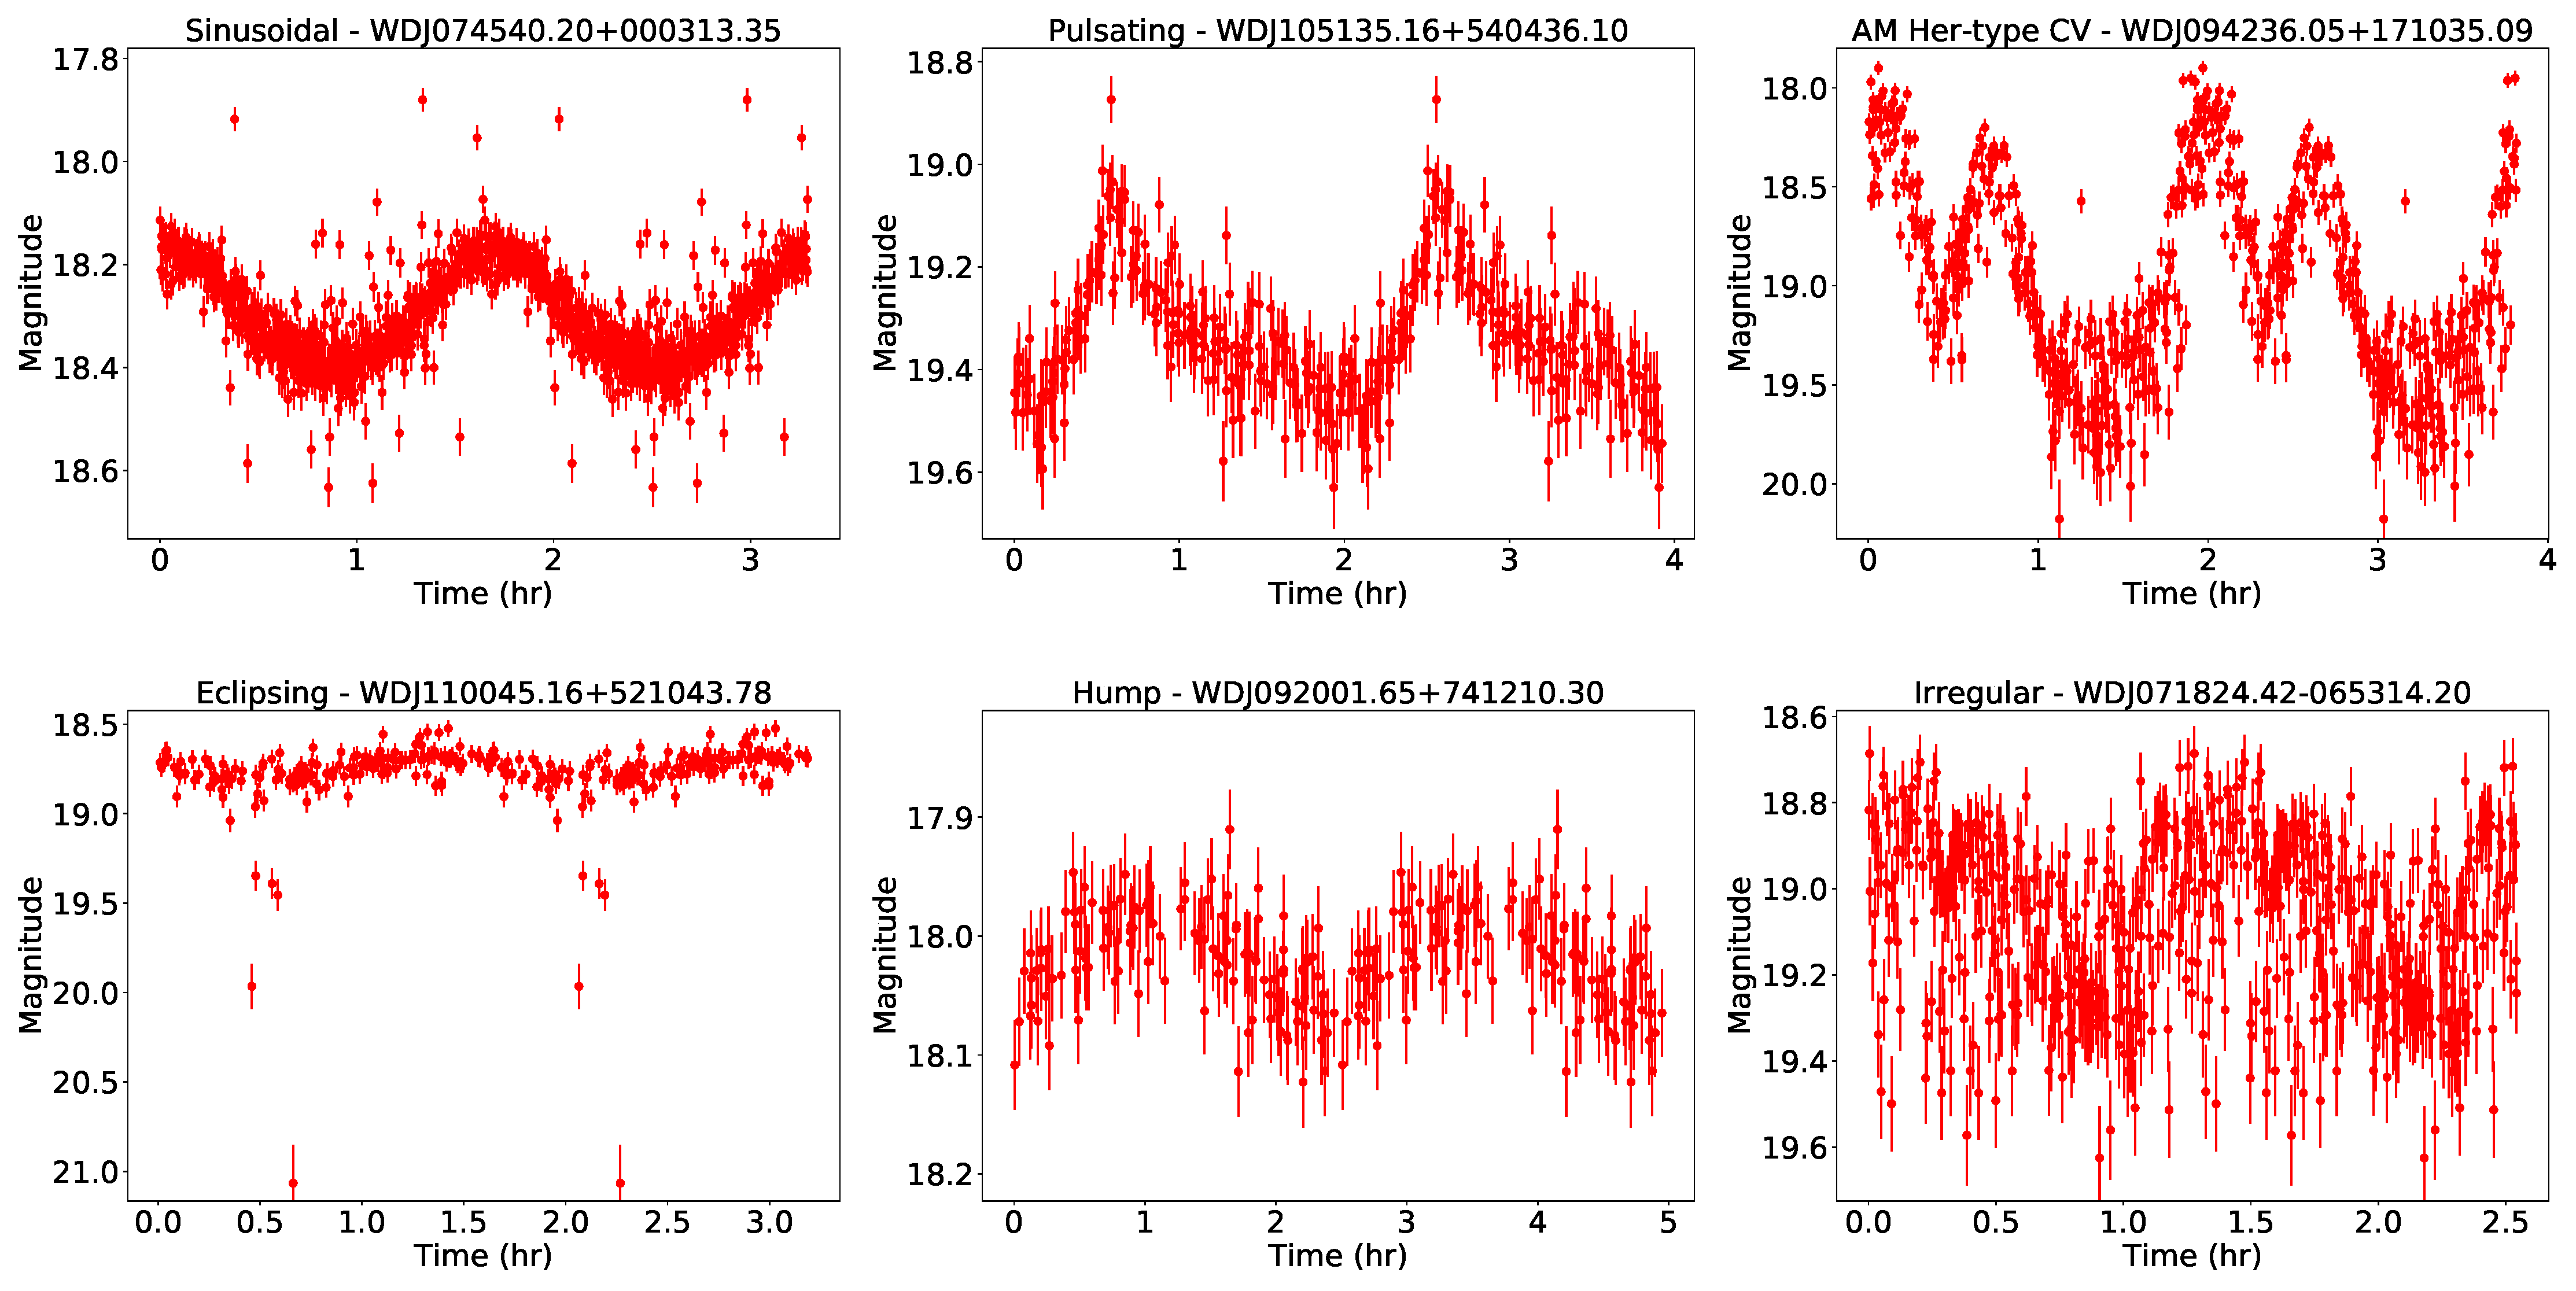
\includegraphics[width=0.9\linewidth]{./Period_Class.eps} 
	\caption{
		Templates for light curve classification.
	}
	\label{fig:2} 
\end{figure}
\begin{figure} 
	\centering
	\includegraphics[width=0.9\linewidth]{./TorqueDensity.png} 
	\caption{
		Torque density of a direct impact system visualized with the Python package \href{https://yt-project.org}{\texttt{yt}},.
	}
	\label{fig:3} 
\end{figure}
 
\end{cvletter}

%----------------------------------------------------------------------------------------

%\makeletterclosing % Print the signature and enclosures

\end{document}